% \usepackage{amsmath,amssymb,amsfonts}
% \usepackage{algorithmic}
% \usepackage{graphicx}
% \usepackage[inline, shortlabels]{enumitem}
% \usepackage{tabularx}
% \usepackage{caption}
% \usepackage[T2A,T1]{fontenc}
% \usepackage[english]{babel}
% \captionsetup{font=it}
% \usepackage{ragged2e}
% \usepackage{hyperref}
% \usepackage{pifont}
% \usepackage{footmisc}
% \usepackage{pdfpages}
% \usepackage{booktabs}
% \usepackage{csquotes}
% \usepackage{smartdiagram}
% \usepackage[inkscapeformat=png]{svg}
% \usepackage{textcomp}
% \usepackage{xcolor}
% \def\BibTeX{{\rm B\kern-.05em{\sc i\kern-.025em b}\kern-.08em
%     T\kern-.1667em\lower.7ex\hbox{E}\kern-.125emX}}
% \usepackage{cite}
% \usepackage{amsmath}
% \newcommand{\probP}{\text{I\kern-0.15em P}}
% % \include{figures/ADTreePreamble}

% \usepackage{etoolbox}
% \patchcmd{\thebibliography}{\section*{\refname}}{}{}{}

% \setlength{\extrarowheight}{2.5pt}

% \renewcommand{\arraystretch}{0.2}


% % \renewcommand{\arraystretch}{1.7}

% \newcommand{\before}[1]{\textcolor{red}{#1}}
% \newcommand{\after}[1]{\textcolor{green}{#1}}

% \newcommand{\old}[1]{\textcolor{orange}{#1}}
% \newcommand{\rem}[1]{\textcolor{red}{#1}}
% \newcommand{\todo}[1]{\textcolor{orange}{\newline \textit{\textbf{TODO:} #1}} \newline \newline }

% \makeatletter
% \newcommand{\linebreakand}{%
%   \end{@IEEEauthorhalign}
%   \hfill\mbox{}\par
%   \mbox{}\hfill\begin{@IEEEauthorhalign}
% }
% \makeatother


\section{Introduction}

% Question : est-il nécessaire de parler autant de l'AICA pour arriver à l'étude de cas avec des agents d'attaques et de défense déployés sur un réseau de nœuds ?
% Contexte

% todo : motiver dans l'intro l'intelligence artificielle : le plan simulé fait appel à différentes techniques : système multi-agent, prise de décision collective, planification, etc. (mind map de l'IA)

\noindent
Le développement de l'Internet des objets a mis en évidence une augmentation de la surface d'attaque des systèmes en réseau, offrant ainsi aux pirates davantage de moyens de s'infiltrer.
Dans ce contexte, le \textquote{AICA IWG}\footnote{Ce groupe de travail (voir \url{https://www.aica-iwg.org/}) a succédé au \textit{Research Task Group IST-152} de l'OTAN, qui se concentrait sur le concept de \textquote{Agents intelligents, autonomes et fiables pour la cyberdéfense et la résilience}.} a poursuivi le développement de l'\textquote{Agent autonome intelligent de cyberdéfense} (AICA).
% Un agent est par définition une entité autonome capable de percevoir son environnement local à l'aide de capteurs et d'agir sur cet environnement à l'aide d'actionneurs~\cite{russell1995modern}.
L'AICA doit pouvoir être déployé de manière autonome sur un système hôte afin de détecter, d'identifier et de caractériser les anomalies/attaques, de développer et de gérer la mise en œuvre de contre-mesures et de dialoguer avec l'extérieur. À cette fin, il est conçu pour être proactif, furtif et capable d'apprendre.

% Objectifs / Motivation pour le simulateur
En outre, compte tenu des cyberdéfenseurs et des cyberattaquants déployés dans une infrastructure réseau dynamique, les questions liées aux stratégies d'action collectives de cyberdéfense constituent des défis pour les outils de modélisation et de simulation.

% Méthode
\noindent
La principale contribution est un modèle de simulation dont l'intérêt principal est de fournir un cadre commun pour mettre en œuvre et évaluer différents types d'agents cyberdéfenseurs et cyberattaquants sur les mêmes environnements en réseau. L'intégration de scénarios d'attaque existants dans les cyberattaquants vise à évaluer l'efficacité des agents, à analyser ou visualiser leurs différents comportements, à former des agents de cyberdéfense contre les agents de cyberattaque, etc. En outre, elle permet de repérer les causes de dysfonctionnements ou de mauvaises performances et d'améliorer les agents cyberdéfenseurs. Bien que cela puisse soulever plusieurs défis liés à l'IA, tels que la génération d'environnements réseau, l'article se concentre particulièrement sur l'apprentissage multi-agents et la prise de décision collective.

% Résultats et conclusion
La section II donne un aperçu des travaux pertinents traitant des aspects de la modélisation des cyberattaquants et des agents de cyberdéfense dans les systèmes hôtes en réseau. La section III présente la modélisation abstraite pour la simulation, sa mise en œuvre technique et son utilisation pour l'intégration et l'évaluation de scénarios d'attaque/défense. Dans la section IV, nous présentons une étude de cas basée sur MITRE ATT\&amp;CK~\cite{MITREATTACKWebiste} et sa mise en œuvre complète dans le simulateur sous la forme d'un scénario d'attaque/défense pour les cyberattaquants et les cyberdéfenseurs. Elle présente également les résultats de l'exécution des scénarios afin d'évaluer la pertinence de la simulation. La section V conclut sur les limites à surmonter et les perspectives d'avenir.

% \rem{On voit pas le lien avec ce qui est dit avant ; Cette section doit faire écho avec ce qui est dit dans l'environnement : modéliser un environnement avec des agents d'attaque/défense, modéliser les attaques/défense, etc.}
% \rem{Pourquoi avoir choisi chacun des éléments pour ces besoins... ?}
% \rem{Utiliser un article déjà publié qui évoque toutes les technologies (Dec-POMDP, ...)}

\section{Travaux connexes sur la modélisation}

\noindent

Peu de travaux traitent directement de la modélisation des cyberattaquants et des cyberdéfenseurs qui s'affrontent dans un système hôte en réseau. En effet, les travaux disponibles sur le sujet proposent principalement une méthode de modélisation des actions d'un cyberattaquant unique dans des scénarios d'attaque spécifiques, tandis que la cyberdéfense est généralement envisagée de manière optionnelle, en réaction.

%\after{À notre connaissance, il n'existe aucun cadre formel qui modélise précisément à la fois les agents collaboratifs attaquants et défenseurs dans un réseau tout en étant indépendant du contexte d'application.}
%Néanmoins, certains travaux fournissent des approches potentielles pour modéliser un environnement de nœuds en réseau et/ou les interactions entre agents.
%De plus, pour de nombreux travaux de modélisation avancés, l'approche multi-agents n'est pas entièrement satisfaite dans le sens où les agents sont conçus à partir de la connaissance de l'ensemble de l'environnement.
% Néanmoins, indépendamment du niveau d'abstraction et du type de support, les travaux considérés pourraient être étendus pour modéliser l'impact des actions des agents cyberattaquants et cyberdéfenseurs sur un environnement en réseau.
% Peu d'autres modélisations proviennent d'approches de simulation ou de réseaux réels par le biais de l'émulation/virtualisation.

\

% \subsection{Graphiques d'attaque}
\noindent
\textbf{Graphiques d'attaque} : \quad Les graphiques d'attaque~\cite{CPhilips1998} sont des représentations graphiques des différentes façons dont un attaquant peut exploiter les vulnérabilités d'un système en réseau. Ils représentent le système comme un ensemble de nœuds (tels que des ordinateurs, des applications ou des connexions réseau) et les attaques possibles comme des arêtes entre ces nœuds. Le graphique montre comment un attaquant peut se déplacer d'un nœud à un autre en exploitant des vulnérabilités et exprime les conséquences sur le réseau~\cite{CPhilips1998}.
Les graphiques d'attaque peuvent être utilisés pour identifier les vulnérabilités les plus critiques d'un système en réseau et aider le défenseur à hiérarchiser ses efforts pour sécuriser ces vulnérabilités dans ce système.

% \subsection{Arbres d'attaque-défense}


\noindent
\textbf{Arbres attaque-défense} : \quad Les arbres attaque-défense~\cite{BKordy2010} (arbres AD) sont des modèles graphiques représentant les objectifs de l'attaquant et les contre-mesures du défenseur sous la forme d'une structure arborescente. Les arbres AD fournissent une représentation plus abstraite du système et des objectifs des attaquants, tandis que les graphiques d'attaque fournissent une représentation plus concrète des composants du système et de leurs relations. La racine de l'arbre représente l'objectif ultime des cyberattaquants. Les sous-nœuds associés aux branches représentent les différentes stratégies d'attaque que l'attaquant pourrait utiliser pour atteindre son objectif. Ils peuvent être accompagnés de contre-mesures préventives ou réactives du défenseur (pare-feu, systèmes de détection d'intrusion, plans d'intervention en cas d'incident, etc.).
Les arbres AD permettent d'identifier les points faibles de la défense d'un système~\cite{BKordy2010}.


\noindent
\textbf{Modélisation par réseaux de Petri} : \quad Les réseaux de Petri pouvant être utilisés pour décrire des processus concurrents, certains travaux ont cherché à modéliser les attaquants et les défenseurs dans un système en réseau.
Les attaques extraites de bases de données peuvent être modélisées à l'aide de réseaux de Petri afin d'intégrer les cyberattaquants et les cyberdéfenseurs, leurs stratégies et le coût de leurs actions, comme dans ~\cite{MPetty2022}. Les réseaux de Petri se révèlent également utiles pour modéliser les attaques par injection de langage de requête structuré afin d'inclure les stratégies des joueurs~\cite{JBland2020}.
Ils sont utilisés comme cadre pour évaluer et comparer plusieurs modèles d'attaque.
Dans ~\cite{SYamaguchi2020}, les préoccupations liées aux logiciels malveillants IoT ont également été abordées pour le logiciel malveillant \textquote{Mirai} à l'aide d'une solution \textquote{white worm} exprimée sous la forme d'un modèle formel avec des réseaux de Petri orientés agents étendus. Cette modélisation permet de simuler un exemple de combat entre le ver white hat et le logiciel malveillant Mirai.


\noindent
\textbf{Modèles de jeu} : \quad Certains travaux ont proposé de modéliser les interactions entre les attaquants et les défenseurs dans un réseau comme des joueurs dans un jeu, où chaque joueur dispose d'un ensemble d'actions qu'il peut effectuer.
Parmi les travaux notables, citons : Panfili et al.~\cite{MPanfili2018}, où un jeu à somme générale multi-agents opposant un attaquant à un défenseur est utilisé pour trouver un compromis optimal entre les actions de prévention et les coûts ; Attiah et al.~\cite{AAttiah2018}, où un cadre théorique de jeu dynamique est proposé pour analyser les interactions entre l'attaquant et le défenseur comme un jeu de sécurité non coopératif ; et Xiaolin et al.~\cite{CXiaolin2008}, qui utilisent des modèles de processus de Markov pour évaluer les risques dans les systèmes en réseau.

\noindent
Certaines approches fondées sur la théorie des jeux s'inscrivent dans le cadre des \textquote{jeux stochastiques partiellement observables} (POSG) ou, plus précisément, dans celui des \textquote{processus de décision markoviens décentralisés partiellement observables} (Dec-POMDP). Les POSG et les Dec-POMDP sont tous deux des cadres de modélisation mathématique des problèmes de prise de décision dans lesquels des agents interagissent entre eux et dans un environnement stochastique~\cite{beynier2010}. Dans un POSG, un groupe d'agents interagit avec un environnement stochastique et partiellement observable. Chaque agent agit en fonction de ses propres observations et d'une politique locale. Les agents peuvent avoir des objectifs différents, car chaque agent a sa propre fonction de récompense et le jeu est généralement supposé être non coopératif~\cite{jk2020}. Dans un Dec-POMDP, plusieurs agents peuvent avoir une fonction de récompense commune et peuvent coordonner leurs actions pour atteindre un objectif commun, notamment en étant capables de communiquer~\cite{bernstein2013}.

\

% \rem{Mettre en perspective les besoins du modèle, ce qui est fait dans la section 2 avec les outils utilisés : Dec-POMDP, etc.}

% \rem{Dans II, c'est l'EDT (ce ne sont pas mes choix, ce qui existe) mais dans III fait les choix}

\noindent
Afin de définir une modélisation, nous avons pris un cas d'utilisation tiré de l'AICA~\cite{theron_autonomous_2021}. Nous nous intéressons à la modélisation d'un environnement réseau composé de \textit{nœuds} sur lesquels des cyberattaquants et des cyberdéfenseurs \textit{agents} peuvent être déployés pour observer et agir. Ces nœuds peuvent être décrits par un ensemble de \textit{propriétés} liées aux processus, aux systèmes de fichiers, aux systèmes d'exploitation, à l'architecture matérielle, etc.
Les \textit{observations} et les \textit{actions} des agents sont conditionnées par leurs propres propriétés (y compris celles qu'ils connaissent) et par des incertitudes. Par exemple, la lecture d'un fichier donné ou le remappage de ports peut nécessiter un niveau de privilège élevé ; ou la réception de données provenant d'un capteur physique n'est pas garantie à tout moment.
Chaque agent qui applique des actions modifie les propriétés d'un ou plusieurs nœuds. Cela modifie l'état de l'environnement, rapprochant ou éloignant les agents de leur objectif.
Les principales caractéristiques de cette description englobent des notions telles que l'incertitude dans les observations, les conditions dans les actions pour la transition d'état et les métriques que nous considérons comme exprimées dans une modélisation Dec-POMDP.
%\after{Ceci vise à répondre au besoin d'un modèle formel d'agents attaquants et défenseurs englobant divers contextes d'application.}

\section{Modèle de simulation}

\subsection{Modélisation générale Dec-POMDP de l'environnement et des agents}

% \rem{Manque d'organisation : modélisation de l'environnement, des agents attaquants, des agents défenseurs, des stratégies de défense/d'attaque, ... On s'attend à une suite, quitte à redécouper...}

\begin{figure*}[]
    \centering
    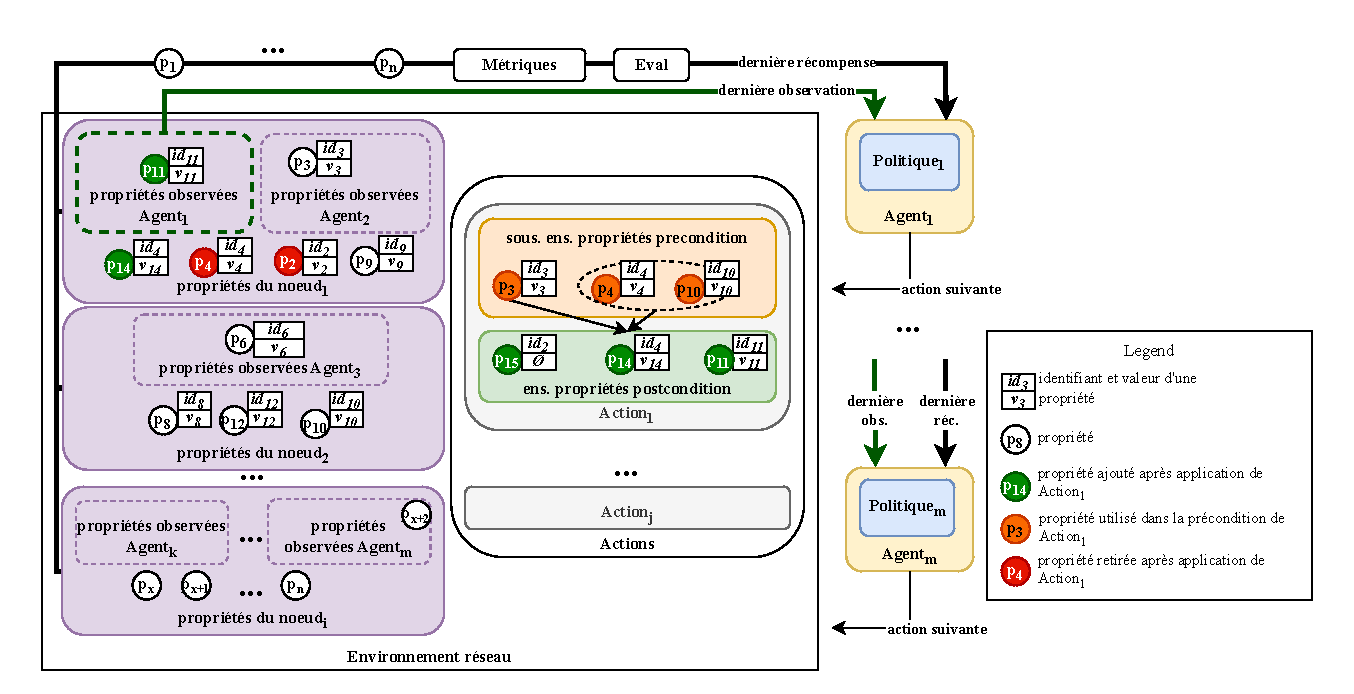
\includegraphics[width=0.97\textwidth]{figures/model_example_illustration.pdf}
    \caption{Vue illustrative du modèle de simulation}
    \label{fig:model_example_illustration}
\end{figure*}

\noindent
D'un point de vue global, le modèle Dec-POMDP proposé exprime l'état d'un environnement comme l'ensemble des propriétés des nœuds, y compris les propriétés observables des agents. Nous définissons une propriété comme un couple composé d'un identifiant et d'une valeur. L'état de l'environnement est modifié lorsqu'une action est appliquée par un agent. Une action ne peut être appliquée que si la condition préalable booléenne basée sur les propriétés est satisfaite dans l'état actuel de l'environnement. L'état résultant est ensuite modifié en fonction de la post-condition, ce qui conduit finalement à l'ajout de certaines nouvelles propriétés et à la suppression d'autres propriétés. Une fois qu'une action a été appliquée avec succès par un agent, les propriétés observables du même agent lui sont renvoyées sous forme d'observations issues de ce nouvel état. Une récompense est également calculée en fonction de l'état actuel et renvoyée à l'agent. Un agent est choisi pour être modélisé comme une fonction de comportement qui doit sélectionner la prochaine action à effectuer en fonction des observations et des récompenses reçues.

Il existe différentes façons d'exécuter plusieurs agents dans un même environnement en ajustant le nombre d'agents à exécuter dans un intervalle de temps et le nombre d'actions à jouer par un agent dans un intervalle de temps. Même si cela n'est pas réaliste, nous avons choisi le \textquote{cycle d'environnement d'agent}~\cite{jk2020} comme première approximation en faisant jouer plusieurs agents une action à chaque tour de manière cyclique et séquentielle. Le cycle d'itération est présenté à travers une vue informelle illustrative du modèle de simulation dans la figure~\ref{fig:model_example_illustration}. Elle montre $i$ nœuds avec leurs propriétés, y compris celles observées par les $m$ agents, et comment chacune des $j$ actions disponibles associe un ensemble de propriétés préalables à un sous-ensemble de nouvelles propriétés à ajouter à l'environnement, en supprimant éventuellement les propriétés obsolètes ayant les mêmes identifiants que les nouvelles propriétés : \begin{enumerate*}[label=\arabic*),itemjoin={;\quad}]     
    \item Un agent choisit une action parmi ses observations précédentes et les récompenses en fonction d'une fonction de comportement. Dans la figure~\ref{fig:model_example_illustration}, lorsque $Agent_1$ commence son premier tour, il ne reçoit que les observations initiales ($p_{1}$) et zéro récompense, et choisit $Action_1$


    
    \item L'environnement est mis à jour par une fonction de transition qui dépend de l'état actuel et de l'action entreprise par l'agent (changement des propriétés une fois que la condition préalable est remplie). Une action est utilisée pour modifier les propriétés de l'environnement en mettant à jour la relation entre les identifiants de propriétés et les valeurs de propriétés.
    Par exemple, dans la figure~\ref{fig:model_example_illustration}, dans l'état actuel, les propriétés de $Node_1$ sont $p_1,p_3,p_4,p_2,p_9$. Lorsque l'action $Action_1$ est appliquée, la relation associe les sous-ensembles $\{p_3\}$ ou $\{p_4, \allowbreak p_{10}\}$ à $\{p_{15}, \allowbreak p_{14}, \allowbreak p_{11}\}$. La condition préalable basée sur les propriétés peut être comprise comme $p_3 \lor (p_4 \land p_{10})$. Comme $p_{15}$ et $p_{14}$ sont identifiés par $ID_4$ et $ID_2$ qui définissent déjà respectivement $p_{2}$ et $p_{4}$, $p_{4}$ et $p_{2}$ sont supprimés et $p_{11}$ et $p_{14}$ sont ajoutés ($p_{15}$ n'est pas ajouté car $id_2$ n'est associé à aucune valeur)


    
    \item Les propriétés observées sont renvoyées à l'agent exécutant actuel pour son prochain tour. Dans la figure~\ref{fig:model_example_illustration}, $p_{11}$ et $p_1$ sont renvoyés après l'application de $Action_1$.

\end{enumerate*}

\noindent
Les agents sont sélectionnés selon un ordre séquentiel. Chacun reçoit les dernières observations et récompenses de son dernier tour (ou simplement l'observation initiale et zéro récompense s'il s'agit de son premier tour) ; il choisit ensuite l'action suivante à jouer lors de son tour actuel. Une fois que le dernier agent a terminé de jouer (par exemple $Agent_m$), les récompenses sont calculées et envoyées aux cyberattaquants et aux cyberdéfenseurs en fonction de l'évaluation des métriques collectées lors du dernier état. Ensuite, les agents jouent à nouveau en suivant le même ordre séquentiel pour une autre itération.


\subsection{Modélisation formelle Dec-POMDP}

Nous définissons les éléments liés aux propriétés des nœuds, des agents et des actions de l'environnement suivant :

\begin{itemize}

    \item $Ag = \{ag_1,..,ag_{|Ag|}\}$ : ensemble des agents (cyberattaquants et cyberdéfenseurs).
    % \begin{itemize}
    %     \item Avec $Attackers \subseteq Ag$ : l'ensemble des agents attaquants
    %     \item Avec $Defenders \subseteq Ag$ : l'ensemble des agents défenseurs
    % \end{itemize}

    \item Nous appelons le couple $p = (id_{j}, v_{j})$ avec $id_j \in {ID}$ et $v_j \in V$, une propriété.
    \begin{itemize}
        \item $ID$ : l'ensemble des identifiants de propriétés indiquant éventuellement comment les propriétés sont organisées dans une structure de données non plate (telle que $PC1.processes.agents.agent1$). Ces identifiants de propriétés peuvent être utilisés pour un chemin d'accès à un fichier, le type de système d'exploitation utilisé dans un nœud, une ligne de commande utilisée par un agent\dots
        \item $V$ : Ensemble des valeurs de propriétés. Celles-ci peuvent inclure le contenu d'un fichier, une description complète du système d'exploitation, le résultat d'une ligne de commande\dots
        % \item $Valeurs : ID \rightarrow \mathcal{P}(V) = \{(id_{j}, V_{j}) \: | \: id_j \in {ID},$ $V_j \in \mathcal{P}(V)\}$ : une bijection associant un identifiant de propriété à l'ensemble des différentes valeurs auxquelles il peut être associé. Par exemple, l'identifiant $ls\_command\_output$ peut être associé aux valeurs suivantes $\{file.txt,\{file.txt,passwd.txt\}\}$
    \end{itemize}

    \item $P_{j} = \{ p_1, .., p_{|P_{j}|} \}$ : l'ensemble des propriétés $p_{l}$ (avec $l \in \{1,..,|P_{j}|\}$) du nœud $j$ ($j \in \mathbb{N} $). Par exemple, ces propriétés peuvent inclure certains identifiants de processus en cours d'exécution, la liste des fichiers d'un dossier, le type de système d'exploitation avec une description, des connaissances spécifiques d'un agent, etc.
    \begin{itemize}
        \item $P = P_1 \cup P_2 .. \cup P_{|P|} $ : Ensemble de toutes les propriétés des nœuds.
    \end{itemize}

    \item $Obs : \mathcal{P}(P) \times Ag \rightarrow \mathcal{P}(P_{Ag}), P_{Ag} \subset P$ : Relation qui associe les propriétés des nœuds et un agent au sous-ensemble de propriétés observées par l'agent.


    
    \item $Action : P_{pre} \rightarrow P_{post}$ : Relation qui associe un sous-ensemble de propriétés implicite dans une pré-condition booléenne conjonctive équivalente ($P_{pre} \subset \mathcal{P}(P)$) à un sous-ensemble de toutes les propriétés de la post-condition ($P_{post} \in \mathcal{P}(P)$). Par exemple, les propriétés $p_1 = (agent\_X\_privilege\_level, \allowbreak root)$, $p_2 = (agent\_X\_accessed\_text\_editor, \allowbreak Vim)$ et $p_3 = (agent\_X\_bashrc\_known\_filepath, \allowbreak /home/user/.bashrc)$ peuvent former une pré-condition ($p_1 \land p_2 \land p_3$) pour associer un nouvel ensemble de propriétés contenant $p4 = (bashrc\_file\_modified\_by\_X\_agent, \top)$. Deux sous-ensembles de pré-conditions peuvent être associés au même sous-ensemble de post-conditions pour modéliser une disjonction booléenne.

    \item $Metrics: \mathcal{P}(P) \times A \rightarrow \mathbb{R}^{n}$ : donne des métriques associées à un ensemble de propriétés et à une action conjointe. Par exemple, le nombre de nœuds encore actifs, les mouvements latéraux, etc.

\end{itemize}


En utilisant la description formelle d'un Dec-POMDP~\cite{OliehoekA16}, nous proposons le modèle suivant :

\begin{itemize}
    \item $S = \{s_1, ..s_{|S|}\}, s_{i} \subseteq P \: et \: 1 \le i \le |S|$ : L'espace des états en tant qu'ensembles de propriétés possibles.

    \item $A_{i} = \{a_{i}^{1},..,a_{i}^{|A_{i}|}\}, a_{i}^j \in Action \: et \: 1 \le j \le |A_i|$ : l'ensemble des actions possibles pour l'agent $i$.

    \item $T$ : Ensemble des probabilités de transition conditionnelles entre les états
    \begin{itemize}
        \item Avec $T(s,a,s') = \probP(s'|s,a)$, la relation qui associe la probabilité d'aller de l'état $s \in S$ à l'état $s' \in S$ sachant que nous avons joué $a = (P^a_{pre} \times P^a_{post}) \in A$ avec $P^a_{pre} \subset \mathcal{P}(P)$ et $P^a_{post} \in \mathcal{P}(P)$
        \item Avec $\probP(s'|s,a) = 0$ si $s$ ne satisfait pas la condition préalable de $a$ (c'est-à-dire $\exists \: P_{pre_s}^{a} \in P_{pre}^{a} \: | \: P_{pre_s}^{a} \not\in \mathcal{P}(s)$).
        \item Avec $s' = (s - \{p_l=(id_l, v_l) \: | \: p_l \in s \: et$ $id_l \in \{id_k \: | \: (id_k, v_k) \in P^a_{post} \: et \: v_k \neq \varnothing\}\}) \cup P^a_{post}$
    \end{itemize}


    
    \item $R : S \times A \rightarrow \mathbb{R}^2 = Eval \circ Metrics$ : La fonction de récompense qui prend un état et une action et associe un indicateur de performance (à l'aide des métriques de l'état) pour les attaquants et les défenseurs.
    \begin{itemize}
        \item Avec $Eval : \mathbb{R}^{n} \rightarrow \mathbb{R}^2$, associe un vecteur métrique à une récompense pour les cyberattaquants et les cyberdéfenseurs.
    \end{itemize}


    
    \item $\Omega_{i} \subset Range(Obs \: | \: \{ (s, ag_i) | s \in S \: et \: ag_i \in Ag \}) \subset P$ : ensemble des propriétés observables pour l'agent $ag_i$. Par exemple, le contenu d'un fichier, la sortie du journal d'une commande, le résultat d'un scan de port, etc.
    \begin{itemize}
        \item $\Omega = \Omega_1 \cup \Omega_2 .. \cup \Omega_{|Ag|} = Range(Obs)$ : Ensemble de toutes les propriétés observables pour tous les agents.
    \end{itemize}

    \item $O$ : Ensemble des probabilités d'observation conditionnelles.
    \begin{itemize}
        \item Avec $O(s',a,o) = \probP(o|s',a)$, la relation qui associe la probabilité d'observer une observation $o \subset \Omega$ à partir de l'état $s' \in S$ induit par $a \in A$
        \item Avec $\probP(o|s',a) = 0$ si l'état $s' \in S$ ne contient pas les propriétés de $o \subset \Omega$ (c'est-à-dire $o \not\in \mathcal{P}(s')$). Par exemple, un agent joue l'action $x\_reads\_a\_log\_file$, ce qui donne lieu à un nouvel état dont une propriété appartenant à la connaissance de l'agent x est $(log\_file\_content\_known\_by\_x, \allowbreak abc)$. Cette propriété sera donc incluse dans les observations renvoyées à l'agent x. 
    \end{itemize}

\end{itemize}


\subsection{Intégration des scénarios d'attaque/défense\label{sec:ad_integration}}

\noindent
D'un point de vue brut, la modélisation formelle Dec-POMDP proposée s'appuie sur des actions pour simuler la manière dont un système en réseau réel réagirait, y compris les vulnérabilités et les contre-mesures appliquées par les agents cyberattaquants et cyberdéfenseurs.

Un premier défi consiste à construire un scénario d'attaque/défense représentatif d'un système en réseau comportant des vulnérabilités afin de permettre de rendre une attaque en reliant les seules informations disponibles (telles que les tactiques, techniques et procédures connues de MITRE ATT\&amp;CK) et en choisissant des contre-mesures de défense pertinentes (issues des mesures d'atténuation de MITRE ATT\&amp;CK) et un environnement de déploiement. Un deuxième défi consiste à établir les actions correspondant au scénario d'attaque/défense. Comme les actions modifient les propriétés de l'environnement, elles ont également un impact sur l'espace des états possibles et les transitions entre ceux-ci.
De plus, lorsque l'on considère un faible niveau d'abstraction, de nombreuses actions simples peuvent permettre de décrire avec précision les changements opérés dans le réseau. Cependant, cela augmente le nombre d'actions, et encore plus le nombre d'états, car ceux-ci sont des combinaisons des effets des actions.

Ces défis sont directement liés aux questions étudiées concernant la génération automatisée de graphiques d'attaque à l'aide de bases de données disponibles intégrant éventuellement des techniques d'intelligence artificielle, comme dans ~\cite{GFalco2018}. Nous n'avons pas l'intention de nous attarder davantage sur ces questions, car elles dépassent le cadre de ce travail.

\

\noindent
\textbf{Approche d'intégration MITRE ATT\&amp;CK} : Nous suggérons une approche manuelle de haut niveau que nous avons utilisée pour intégrer les informations MITRE ATT\&amp;CK sous forme d'arborescence AD, car elle formalise les actions à jouer dans un scénario et leurs interactions avec l'environnement. Elle vise à aider à établir les actions d'attaque/défense qui seront finalement intégrées dans le simulateur :
\begin{enumerate*}[label=\arabic*),itemjoin={;\quad}]

    \item Pour une menace persistante avancée (APT) donnée, nous avons identifié les tactiques, techniques et procédures pertinentes de MITRE ATT\&amp;CK qui semblaient pertinentes pour un système en réseau


    
    \item Nous avons produit une description reliant les tactiques identifiées entre elles et les techniques, sous-techniques et procédures associées afin de créer un scénario décrivant comment le groupe APT pourrait attaquer le système en réseau. Cette étape définit la topologie du réseau avec ses principales propriétés
    %(telles qu'un réseau d'entreprise composé de plusieurs serveurs de bases de données dédiés communiquant via FTP et HTTP, etc.)

    \item Nous avons créé une arborescence AD comme proposé dans ~\cite{BKordy2010} avec les tactiques comme objectifs d'action principaux et les techniques, sous-techniques et procédures dans la partie inférieure de l'arborescence. Nous avons veillé à disposer de plusieurs chemins pour atteindre un même objectif d'action principal. Nous avons pris soin de définir chaque action d'attaque avec des conditions préalables et des conditions postérieures basées sur les propriétés de l'environnement

    \item Nous avons extrait les techniques/sous-techniques MITRE ATT\&amp;CK liées à la détection et aux mesures d'atténuation que nous avons ajoutées dans l'arbre AD afin d'enrichir les nœuds d'attaque. Nous avons veillé à définir chaque action de défense avec des conditions préalables et des conditions postérieures basées sur des propriétés dans l'environnement.



    % \item Nous avons également répertorié et défini les principales actions environnementales spécifiques au déploiement à partir de la description précédente de l'environnement de déploiement ou des actions d'attaque/défense étendues qui sont communes aux cyberdéfenseurs et aux cyberattaquants. Cette étape permet d'obtenir un environnement plus réaliste, fournissant un nombre représentatif d'actions plausibles qu'un agent peut choisir dans de nombreux systèmes.
    % Ces actions communes pourraient inclure au moins :
    % \begin{itemize}
    %     \item Lecture et écriture de fichiers
    %     \item Créer, supprimer, copier, déplacer, renommer, modifier les propriétés des fichiers/dossiers.
    %     \item Accéder à un dossier, accéder au dossier parent
    %     \item Sélectionner un fichier/dossier pour y appliquer des actions ultérieures
    %     \item Exécuter un fichier binaire
    %     \item Utilisation d'un protocole réseau (tel que HTTP, FTP, SSH, etc.).
    %     \item Autres interactions avec les lignes de commande de base concernant la surveillance ou le contrôle du système.
    % \end{itemize}
    % Ensuite, les propriétés environnementales associées doivent décrire un système de fichiers, une interface de terminal, un port avec des règles, les propriétés des paramètres du système d'exploitation, etc.

\end{enumerate*}

\subsection{Mise en œuvre du modèle de simulation}

\noindent
Les travaux potentiels pour mettre en œuvre notre modèle comprennent : NeSSi2~\cite{DGrunewald2011}, une plateforme de simulation basée sur des agents visant à modéliser uniquement la description au niveau des paquets d'un système en réseau et les effets des attaques DDoS ; et Kotenko et al.~\cite{IKotenko2007}, qui s'appuie sur OMNet++~\cite{Varga2010} pour modéliser et simuler des agents de cyberdéfense coopératifs contre les attaques réseau, en combinant la simulation d'événements discrets, l'approche multi-agents et la simulation au niveau des paquets des protocoles réseau.
% De plus, pour pallier le manque de réalisme, des émulateurs utilisant des machines virtuelles et intégrés à des outils offensifs ont été développés, tels que DCAFE~\cite{GRush2014} et SVED~\cite{HHannes2016}.
Cependant, parmi ceux-ci, aucun ne peut pleinement répondre à la fois à la prise en compte d'un environnement cyber multi-agents pour un modèle Dec-POMDP
%et le besoin d'accessibilité du code (code source ouvert).

\begin{figure}
    \centering
    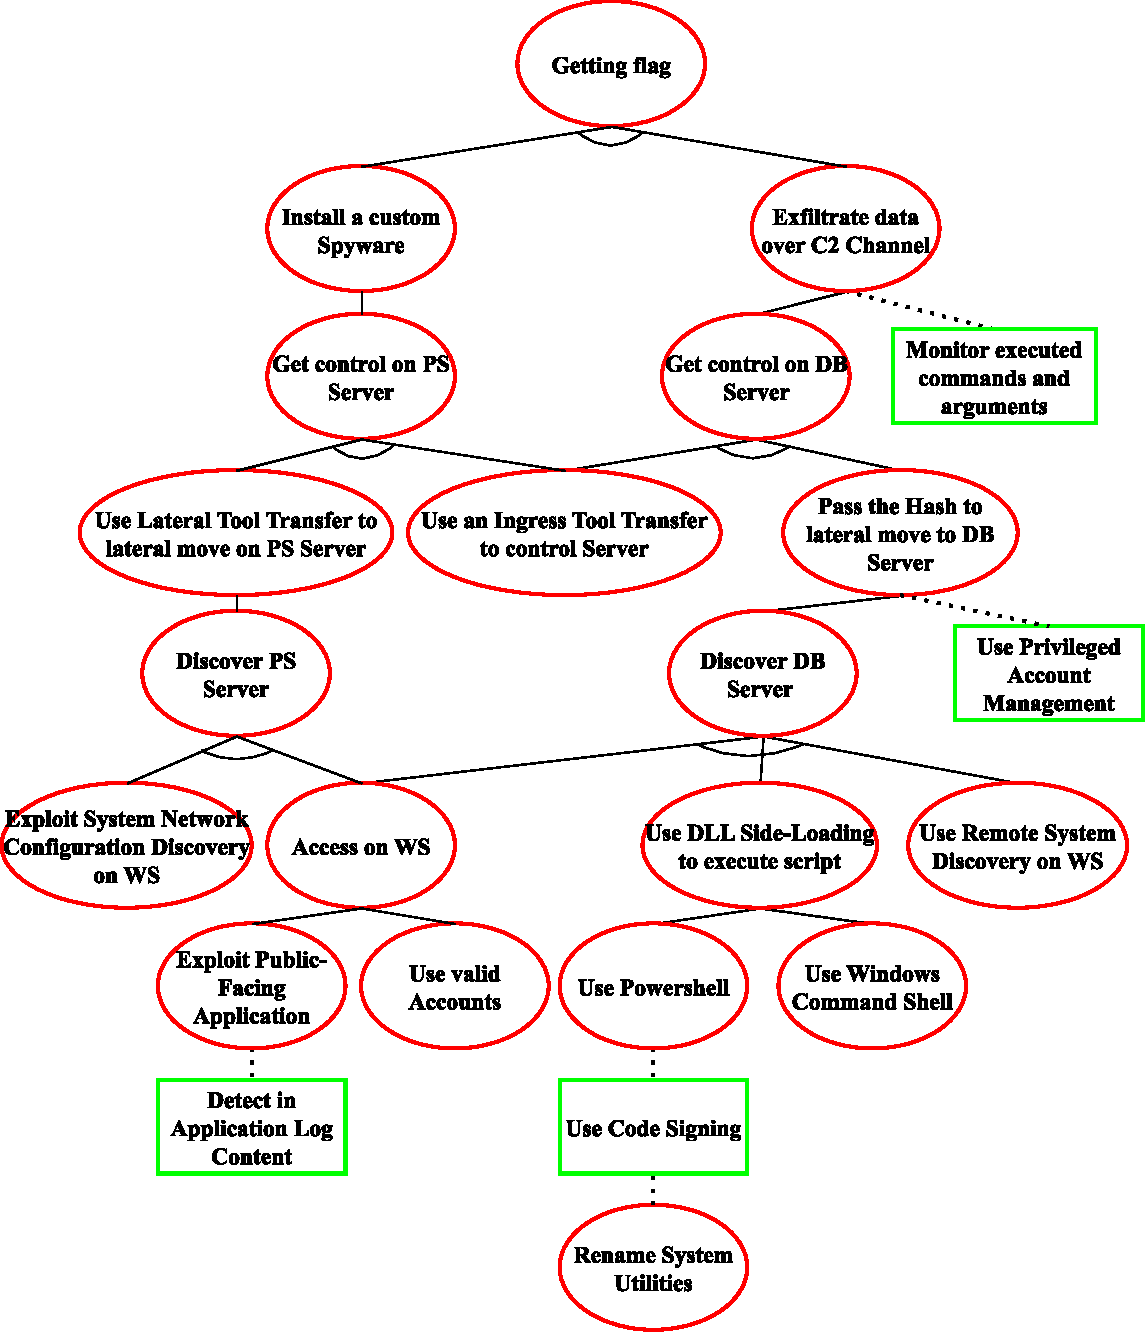
\includegraphics[width=\linewidth]{figures/ADTree.pdf}
    \caption{Aperçu de l'arborescence AD proposée pour l'attaque/la défense}
    \label{fig:ADTree}
\end{figure}

Cependant, nous avons identifié des simulateurs d'événements discrets avec un seul cyberattaquant, tels que CYST\cite{drasar_session-level_2020} ou CyberBattleSim~\cite{cyberbattlesim}, qui fournissent tous deux une simulation de réseau et une approche d'évaluation adaptées à la mise en œuvre de notre modèle, car leurs modèles sous-jacents peuvent être étendus à plusieurs agents. Inspirés par ces approches, nous avons utilisé \textit{PettingZoo}~\cite{jk2020} comme plateforme fondamentale pour implémenter notre modèle Dec-POMDP sur lequel nous avons cherché à implémenter un réseau simulé. \textit{PettingZoo} fournit un cadre dans lequel le concepteur dispose d'outils pour faciliter la mise en œuvre de l'espace d'observations, des actions, de la gestion des agents à chaque tour et des récompenses associées.

% \begin{figure}
%      \centering
%      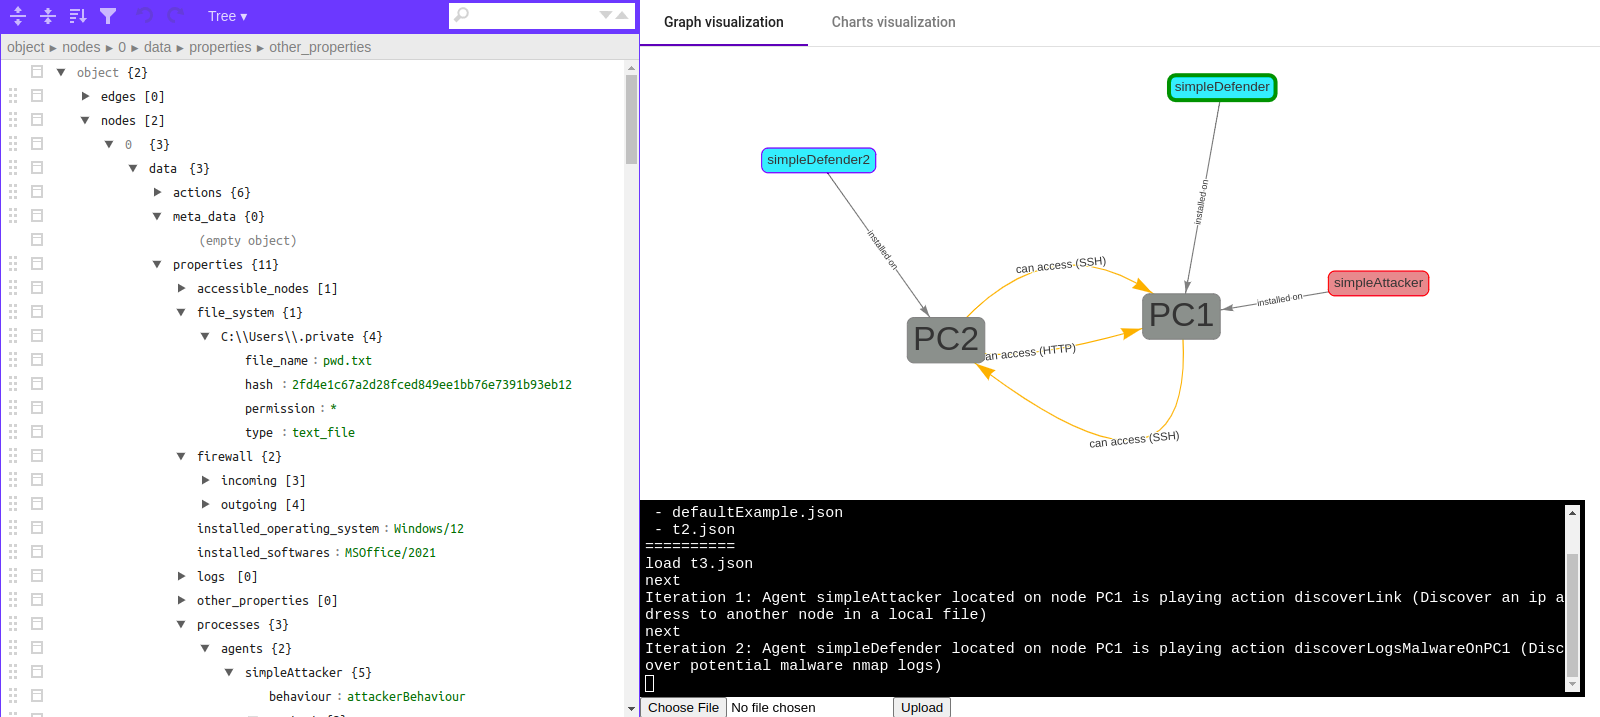
\includegraphics[width=\linewidth]{figures/interface_MCAS.png}
%      \caption{Aperçu de l'interface du simulateur}
%      \label{fig:simulator_interface}
% \end{figure}

Le développement de notre modèle a abouti au simulateur \textquote{Multi Cyber Agent Simulator} (MCAS)~\cite{MCASWebsite}. Dans son état actuel, ce simulateur permet de charger/enregistrer un fichier \textit{json} décrivant les propriétés des nœuds et les actions de l'environnement, ainsi que les agents définis et leurs comportements ; il permet également de lancer l'exécution des agents de cet environnement en mode tour à tour via le terminal. Il est possible de visualiser les propriétés de l'environnement en temps réel et de représenter l'environnement sous forme de graphique. Des métriques sont également affichées.



\section{Étude de cas basée sur MITRE ATT\&amp;CK}

% \rem{Expliquer pourquoi on veut tester les capacités du simulateur -&gt; illustration de comment fonctionne le simulateur}
% \rem{Gallium APT, pourquoi ce choix ? Pourquoi cette étude de cas inspirée de cela ? Qu'est-ce qui est intéressant dans Gallium APT ? Type d'attaque/ coordination d'attaque ?}

\noindent
Dans le but d'évaluer les attaques coordonnées et la défense collective, nous avons choisi GALLIUM APT (un groupe de cyberespionnage actif depuis 2012), car il permet de définir plusieurs attaques simultanées.


\subsection{Topologie du réseau}

% \rem{Pour chaque élément présent dans la figure, faire le lien avec les éléments cités dans la présentation de la topologie...}

\noindent
Sur la base de certaines tactiques GALLIUM APT, nous avons sélectionné quelques techniques/sous-techniques associées afin de proposer un environnement réseau similaire à celui d'une petite entreprise, présenté dans la figure~\ref{fig:scenario_network_topology}. Il est divisé en 5 sous-réseaux communiquant via des routeurs implicites positionnés après un pare-feu :
Le sous-réseau extérieur utilisé pour représenter les attaquants externes comme s'ils se trouvaient sur le même réseau, pour plus de commodité. Il comprend deux ordinateurs de bureau (At1 et At2).
Le sous-réseau DMZ (zone démilitarisée) sert à séparer les appareils accessibles depuis Internet du reste du réseau de l'entreprise. Les serveurs de la DMZ comprennent un serveur web (WS), un serveur de messagerie (ES), un serveur VPN (VPN) et un serveur FTP (FTP), tous connectés de manière bidirectionnelle à l'extérieur et à l'intérieur du réseau de l'entreprise.
Le premier sous-réseau local (ACC) sert à connecter les appareils au sein du service comptable de l'entreprise où travaillent les employés. Il comprend deux postes de travail d'employés (E1 et E2) et un poste de travail du directeur technique (CTO), tous connectés de manière bidirectionnelle à la DMZ. % et uniquement accessible depuis SRV (défini ci-dessous) ;
Le deuxième sous-réseau local (MAR) sert à connecter les appareils au sein du service marketing de l'entreprise. Il comprend un serveur d'impression (PS), un poste de travail d'employé (E3) et une tablette (TAB) connectés via un point d'accès sans fil, tous connectés de manière bidirectionnelle à la zone DMZ. % et uniquement accessibles depuis SRV (défini ci-dessous) ;
Le troisième sous-réseau local (SRV) sert à connecter les appareils de l'entreprise qui fournissent des services. Il contient un serveur API (API), un serveur de base de données (DB) et un contrôleur de domaine (DC).

\begin{figure}
    \centering
    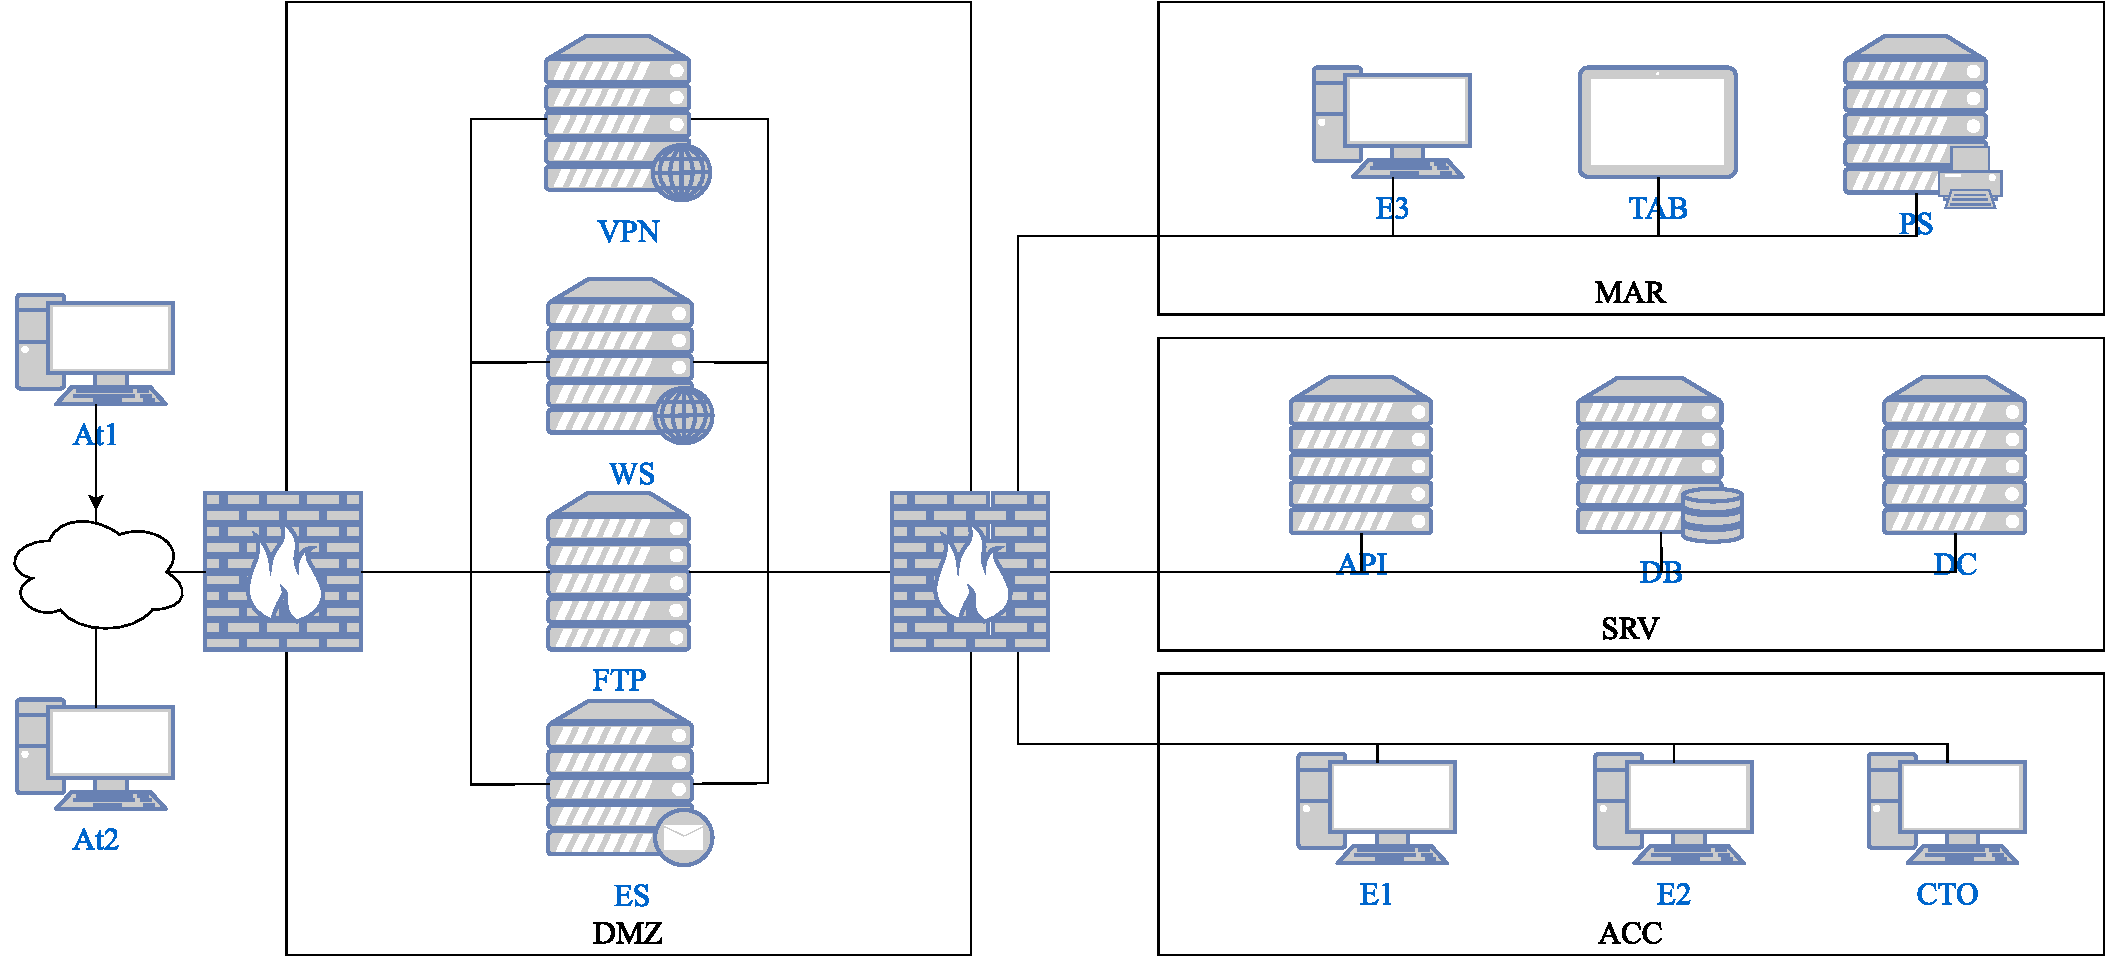
\includegraphics[width=\linewidth]{figures/topology.pdf}
    \caption{Topologie réseau proposée pour une petite entreprise}
    \label{fig:scenario_network_topology}
\end{figure}


%Ces appareils sont accessibles depuis la zone DMZ et depuis le CTO. L'API est également accessible via un tunnel VPN depuis l'extérieur.

% Les machines simulées sont remplies de fichiers, de dossiers, de règles de pare-feu, de services réseau, etc., afin que les attaquants et les défenseurs puissent disposer de plus d'actions pour interagir.


\subsection{Scénario et mise en œuvre des agents avec évaluation}

\begin{figure}
    \centering
    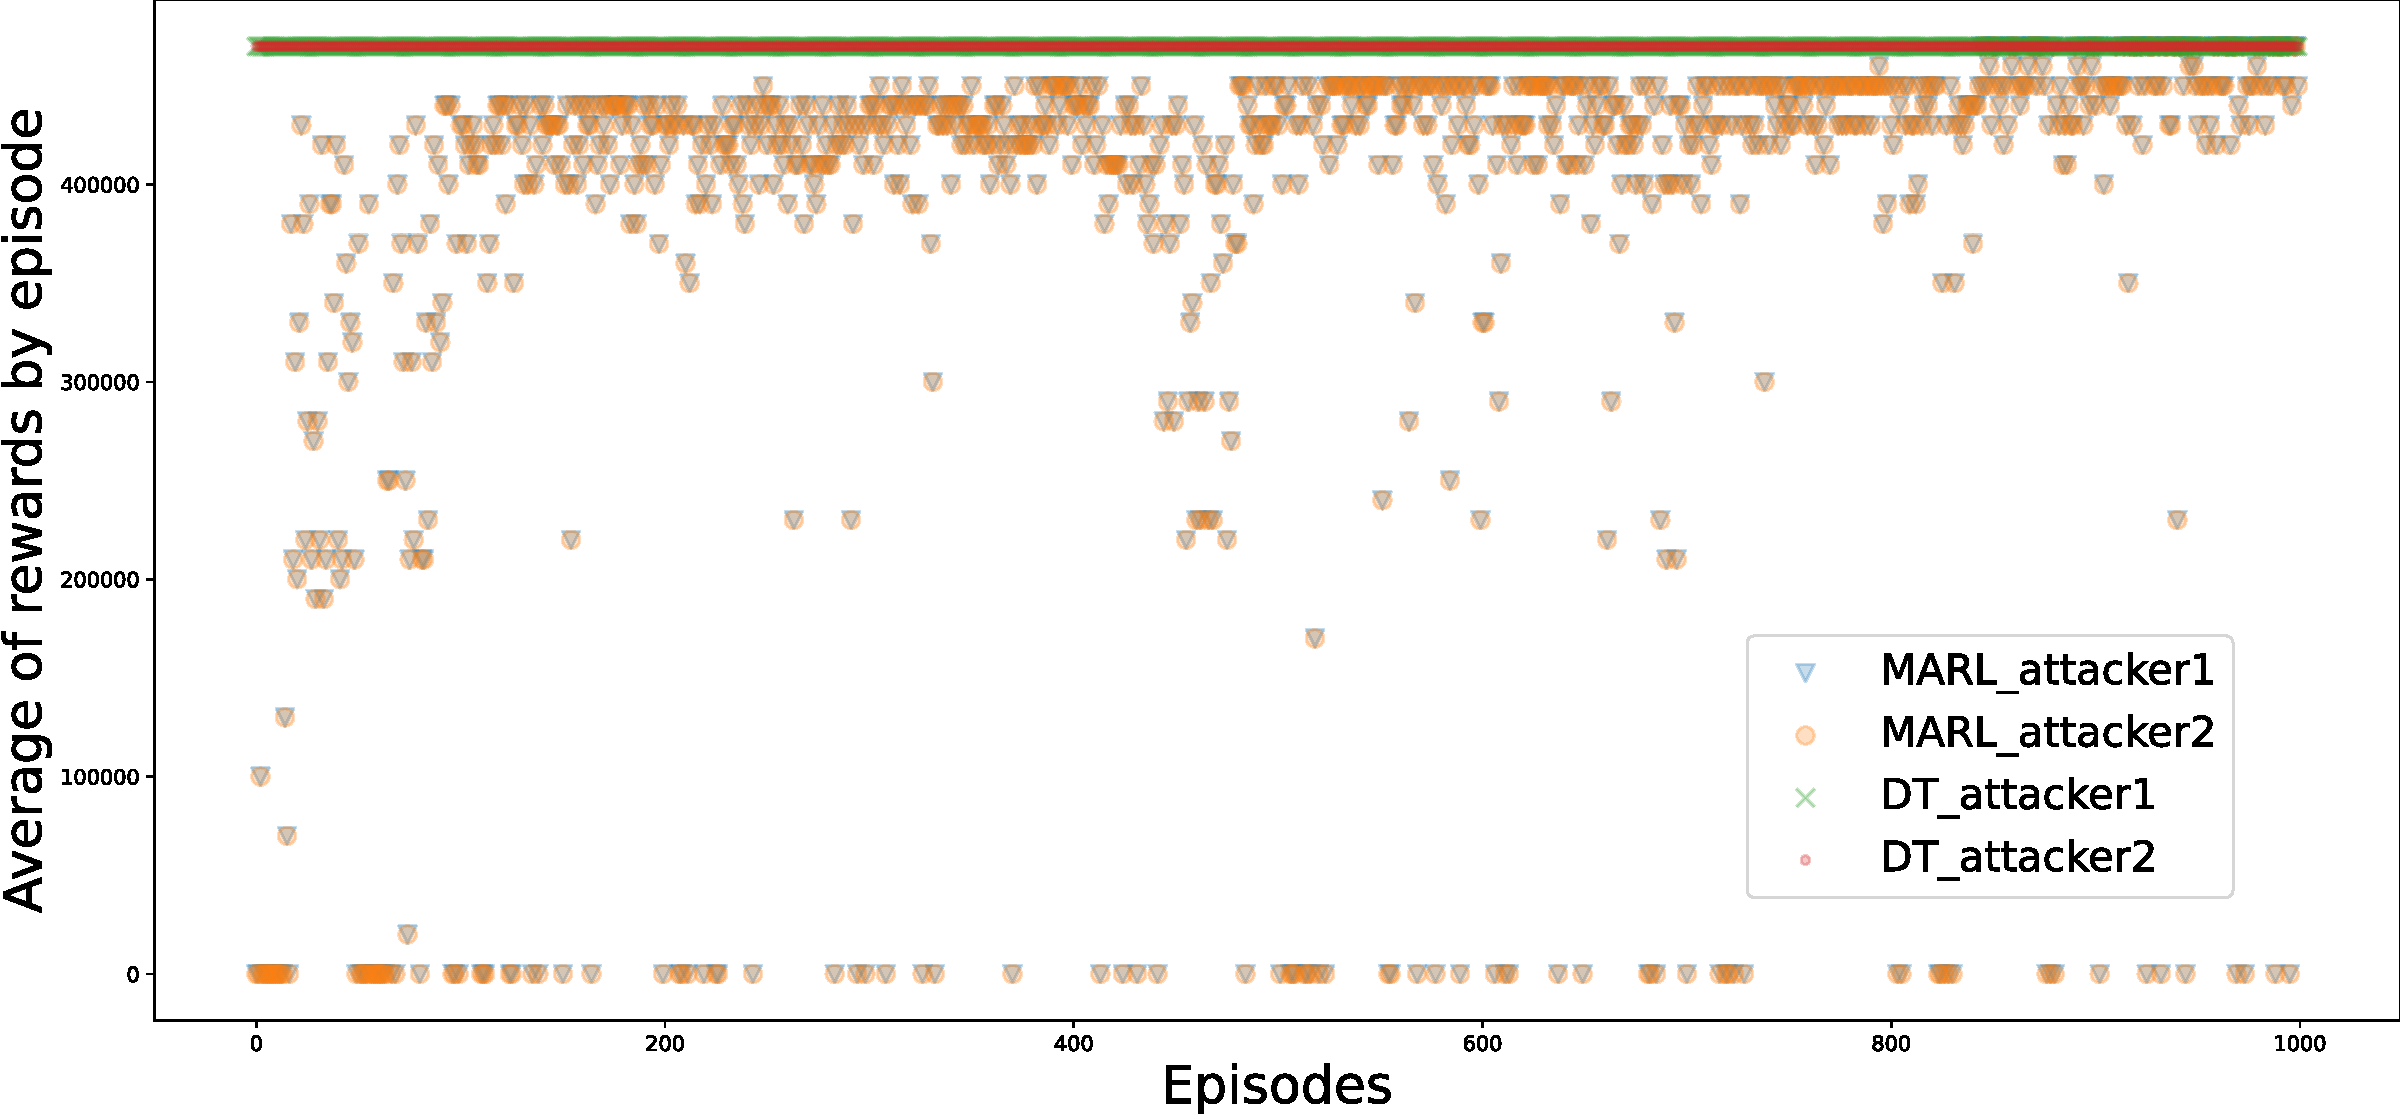
\includegraphics[width=\linewidth]{figures/graphs.pdf}
    \caption{Évolution de la moyenne des récompenses en fonction des épisodes dans des tests à petite échelle avec MARL et des approches par arbre de décision avec cyberdéfense inactive
    }
    \label{fig:graphs}
\end{figure}

\noindent
Les agents cyberattaquants sont initialement déployés sur At1 et At2, tandis que les agents cyberdéfenseurs sont déployés sur WS et DB. L'objectif ultime des attaquants est d'obtenir des données du serveur DB et d'installer un logiciel espion sur le serveur d'impression PS. Conformément à notre approche dans ~\ref{sec:ad_integration}, nous proposons une arborescence AD présentée dans la figure~\ref{fig:ADTree}. Elle montre uniquement les chemins que doivent suivre les attaques pour atteindre leur objectif final, tandis que les actions des défenseurs peuvent les empêcher à plusieurs étapes de l'attaque.
Nous nous sommes d'abord intéressés à la configuration des deux comportements des cyberattaquants, puis à ceux des deux cyberdéfenseurs. Nous avons simulé une version abstraite du scénario sur 1 000 épisodes.

% En outre, nous avons mis en œuvre d'autres actions courantes pour interagir avec le système de fichiers, la configuration du système d'exploitation, la configuration du pare-feu et les services réseau. Ces actions peuvent être dérivées des actions d'attaque/défense, mais ne sont pas implicitement représentées dans l'arbre AD. Elles sont toutefois prises en compte dans la simulation afin que les agents puissent explorer les chemins d'action, même si ceux-ci ne mènent pas à l'objectif final de l'attaquant.


%\subsection{Exécution et évaluation du scénario}

\noindent
\textbf{Approche aléatoire} : \quad L'agent aléatoire choisit ses actions en explorant l'ensemble de l'espace d'action sans aucun critère jusqu'à ce qu'il atteigne l'objectif. Dans notre étude de cas, le chemin d'action le plus court permettant aux attaquants d'atteindre l'objectif final comprend 16 actions différentes parmi les 30 actions définies, ce qui correspond à une faible probabilité de $(1/30)^{16}$.
Cette approche permet d'obtenir un benchmark des cas de défaillance inattendus et de les comparer avec d'autres types d'agents.

\noindent
\textbf{Approche par arbre de décision (DT) } : \quad L'arbre de décision a été appliqué afin d'obtenir une référence lorsque les cyberattaquants ou les cyberdéfenseurs connaissent déjà la meilleure action à entreprendre, le rôle de chaque agent étant défini par un DT.
Dans la figure~\ref{fig:graphs}, $DT\_attacker1$ suit un chemin d'action pour atteindre l'objectif d'installer un logiciel espion personnalisé dans PS. Dans le même temps, $DT\_attacker2$ atteint l'objectif d'exfiltrer des données dans DB et de terminer le chemin d'action en obtenant le drapeau. Nous avons ensuite ajouté les défenseurs $DT\_defender1$, qui doit détecter les journaux malveillants sur WS, et $DT\_defender2$, qui doit utiliser la gestion des comptes privilégiés ou surveiller les commandes et arguments exécutés sur DB. Nous avons observé que les attaquants étaient incapables d'atteindre leur objectif final.

\noindent
\textbf{Approche d'apprentissage par renforcement multi-agents (MARL)} : \quad L'apprentissage Q~\cite{CWatkins1992} a été appliqué avec un apprentissage par programme afin que les attaquants apprennent d'abord comment atteindre l'objectif final de l'attaque avant d'ajouter des défenseurs.
Dans la figure~\ref{fig:graphs}, $MARL\_attacker1$ et $MARL\_attacker2$ suivent le même comportement, affinant finalement les actions appliquées pour atteindre l'objectif final. Après plusieurs épisodes, les chemins d'action choisis par les attaquants ont tendance à être aussi efficaces que les chemins DT. Lorsque nous avons ajouté les défenseurs $MARL\_defender1$ et $MARL\_defender2$, nous avons vérifié que les attaquants étaient de moins en moins capables d'atteindre l'objectif ultime.


\section{Conclusion et perspectives}

\noindent Nous avons proposé une modélisation Dec-POMDP des nœuds en réseau susceptibles d'être attaqués et défendus par des agents. Ce modèle vise à intégrer différents scénarios. La mise en œuvre de ce modèle a conduit à un simulateur dont certaines capacités ont été évaluées à travers un scénario MITRE ATT\&amp;CK. À l'aide de trois approches, nous avons brièvement vérifié comment les approches par arbre de décision, aléatoire et par apprentissage par renforcement peuvent être appliquées à un agent à des fins de comparaison.
Soucieux de tirer parti de cette approche de simulation pour aborder des problèmes réalistes liés aux cyberdéfenseurs, en particulier dans le contexte de l'AICA, nous avons identifié les principales limites à surmonter :
automatiser l'intégration de scénarios plus réalistes en s'appuyant sur une base d'actions et de propriétés communes afin que les agents puissent explorer et agir comme dans des systèmes d'information apparemment similaires à la réalité ;
mettre en place un moyen d'utiliser les avantages des résultats obtenus avec les simulations pour des systèmes émulés ou réels tout en conservant les comportements des agents lors du déploiement ;
améliorer la coordination entre les agents, par exemple en créant plusieurs points d'entrée ou scénarios nécessitant une communication pour atteindre un objectif ;
et introduire de nouvelles contraintes dans les actions (telles que le coût, la durée d'exécution, etc.).
